\subsection{Интерфейс программного средства}

В интерфейсе программного средства имеются общие для всех страниц компоненты: панель настроек, навигационная панели. Помимо общих
элементов, сущесвуют и частные, которые описаны далее.

\subsubsection{Страница регестрации}

Страница регистрации -- первая страница с которой сталкивается новый пользователь при входе в систему.
Форма регистрации состоит из следующих компонентов:
\begin{itemize}
    \item заголовок;
    \item форма регистрации;
    \item меню действий
\end{itemize}

Рассмотреть страницу регистрации можно на рисунке \ref{fig:register}.

\begin{figure}[ht]
    \centering
    \fbox{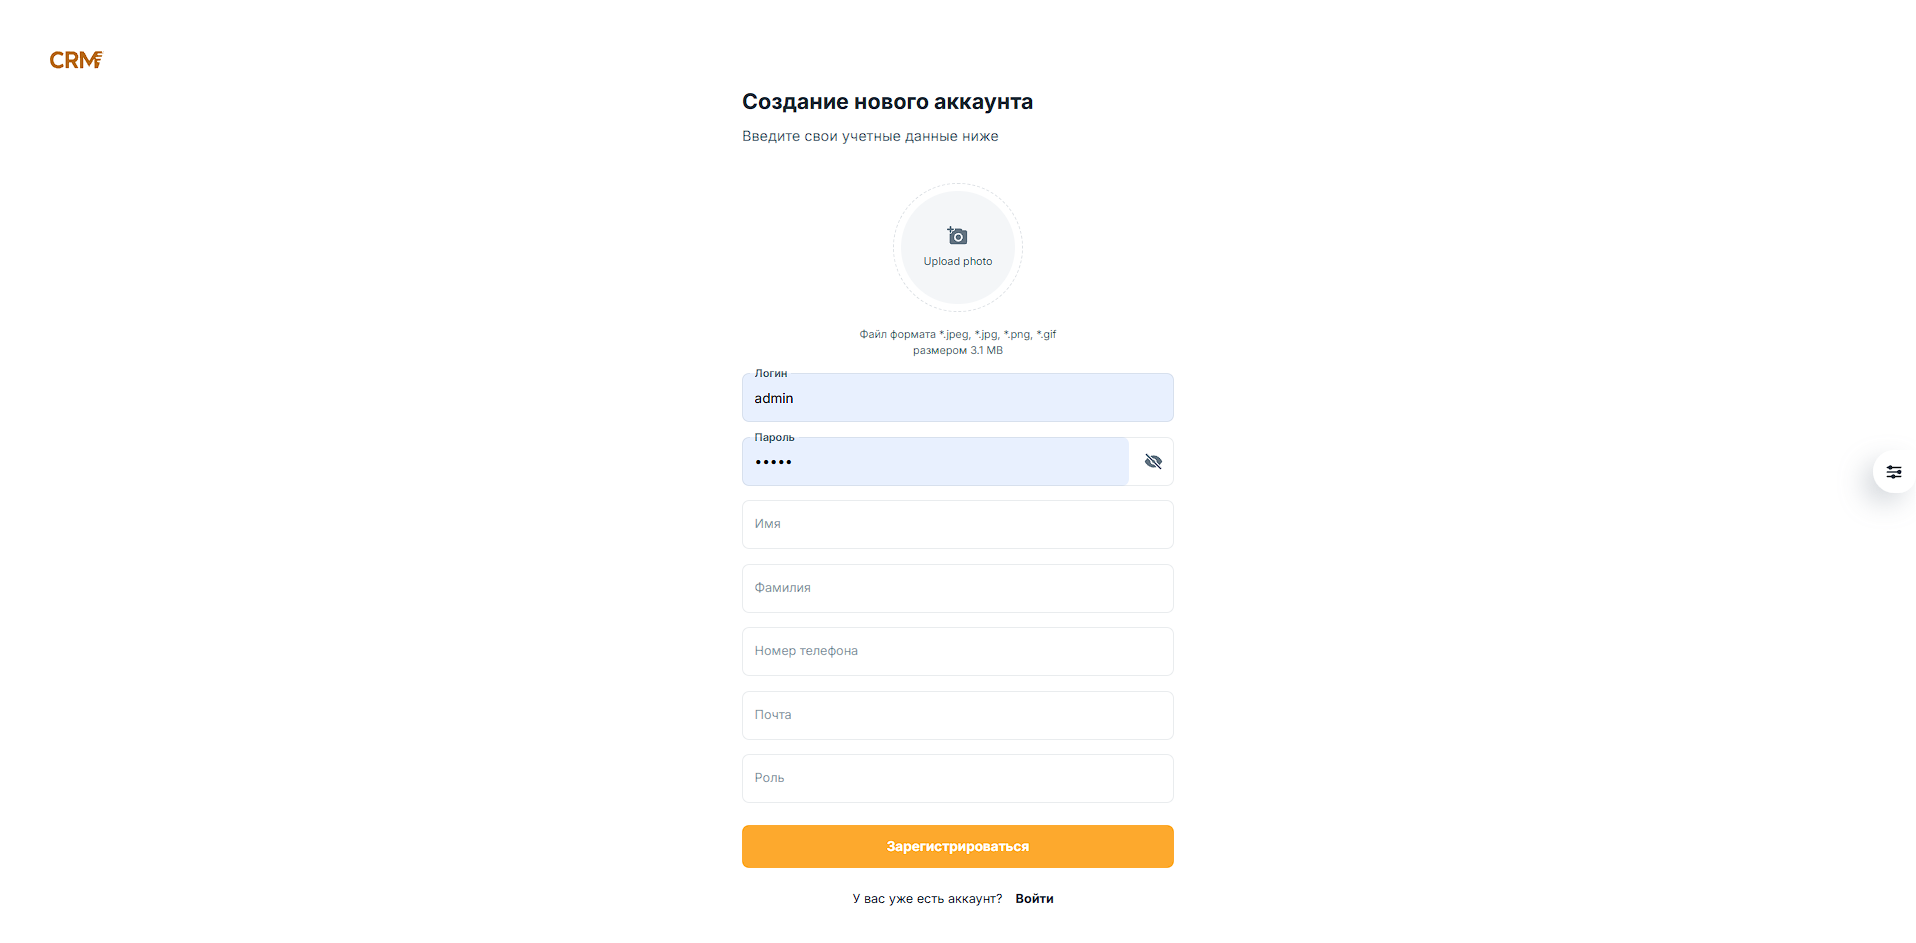
\includegraphics[width=0.75\linewidth]{\commonSecPathPrefix/sec_5/content/register.png}}
    \caption{Страница регестрации}
    \label{fig:register}
\end{figure}

Заголовок информирует пользователя о том, что за страница открыта и описывает действия, которые необходимо выполнить. Форма регистрации 
содержит в себе необходимые поля для создания нового пользователя и кнопку отправки формы регистрации. Меню действий необходимо, чтобы
перейти на страницу входа, на случай, если пользователь попал на страницу регистрации случайно.

\subsubsection{Профиль пользователя}

Профиль пользователя -- страница на которой можно узнать всю информацию о любом пользователе в системе. Владелец аккаунта может изменить
свою контактную информацию на странице профиля пользователя.

Страница пользователя состоит из следующих частей:
\begin{itemize}
    \item шапка страницы;
    \item меню;
\end{itemize}

Внешний вид страницы профиля пользователя можно увидеть на рисунке \ref{fig:profile}.

\begin{figure}[ht]
    \centering
    \fbox{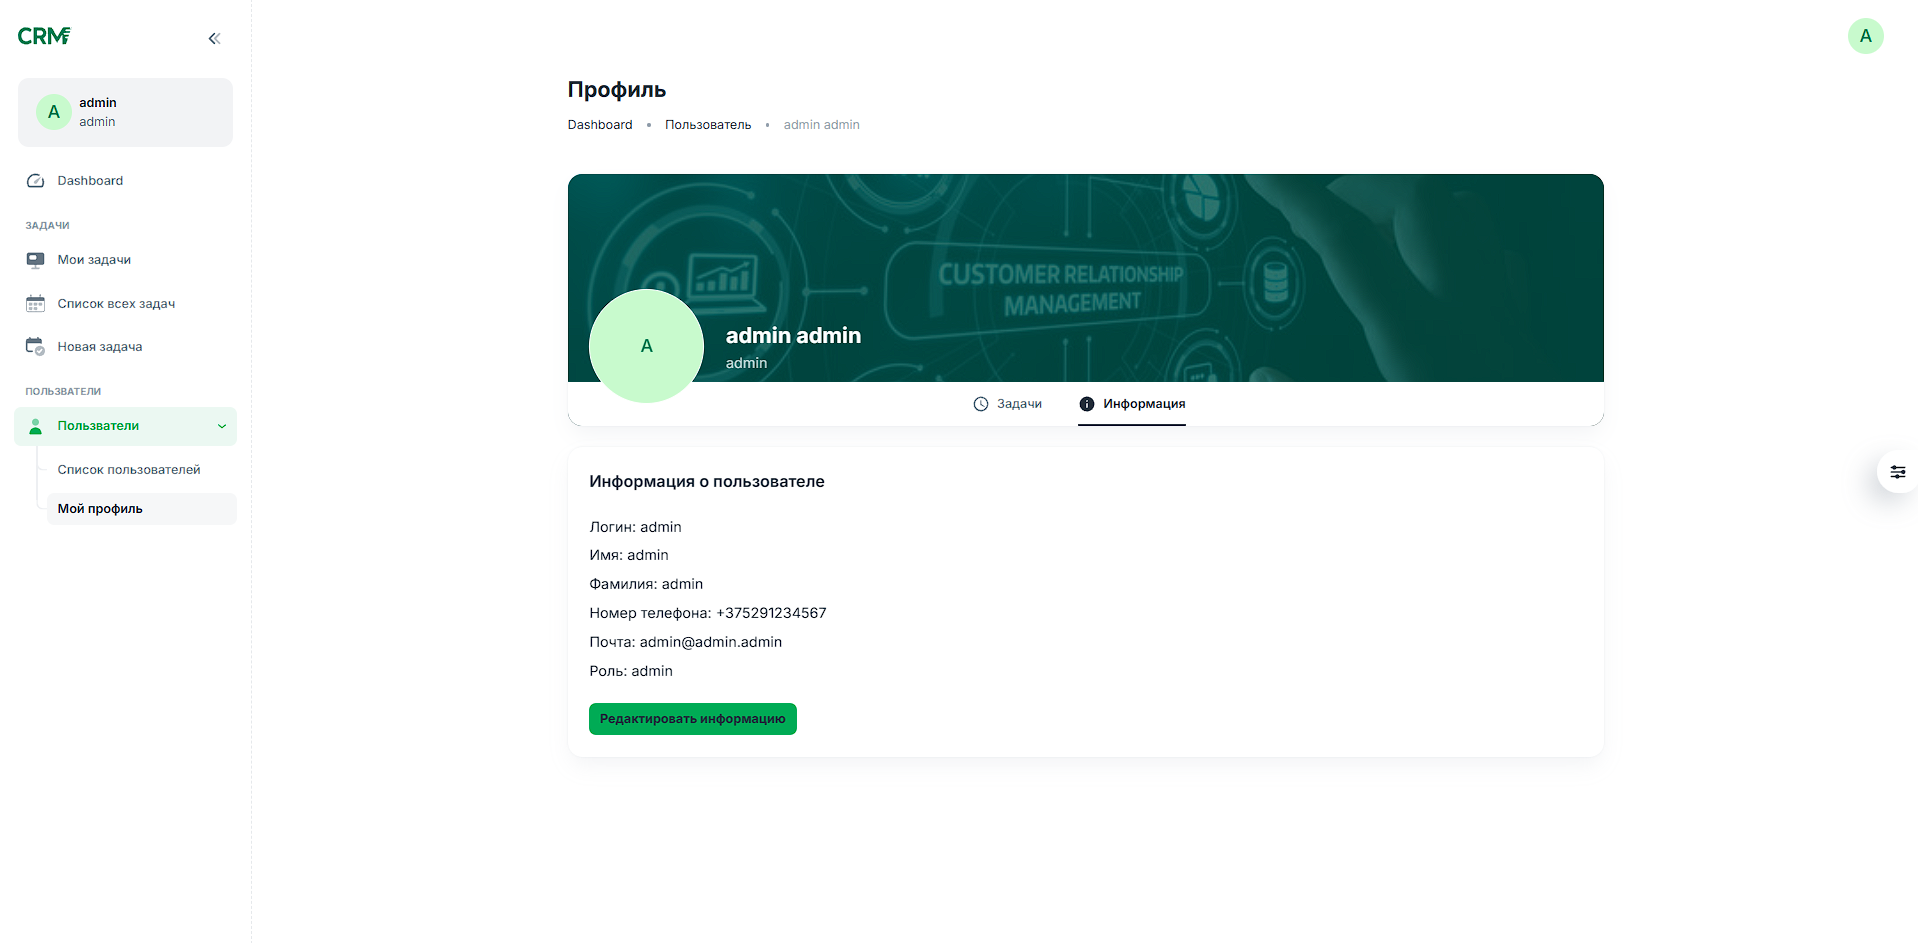
\includegraphics[width=0.75\linewidth]{\commonSecPathPrefix/sec_5/content/profile.png}}
    \caption{Страница профиля пользователя}
    \label{fig:profile}
\end{figure}

Шапка страницы показывает аватар, имя и роль пользователя. Навигационная панель позволяет пользователю выбрать, какую информацию
необходимо вывести. Меню состоит из двух блоков: Задачи, Информация.

\subsubsection{Страница создания задачи}

Страница создания задачи является основной в программном средстве. Основные элементы из которых состоит страница:
\begin{itemize}
    \item основные поля задачи;
    \item блок добавления пользователей;
    \item блок прикрепления файлов;
\end{itemize}

Рассмотреть страницу создания задачи можно на рисунке \ref{fig:task}.

\begin{figure}[ht]
    \centering
    \fbox{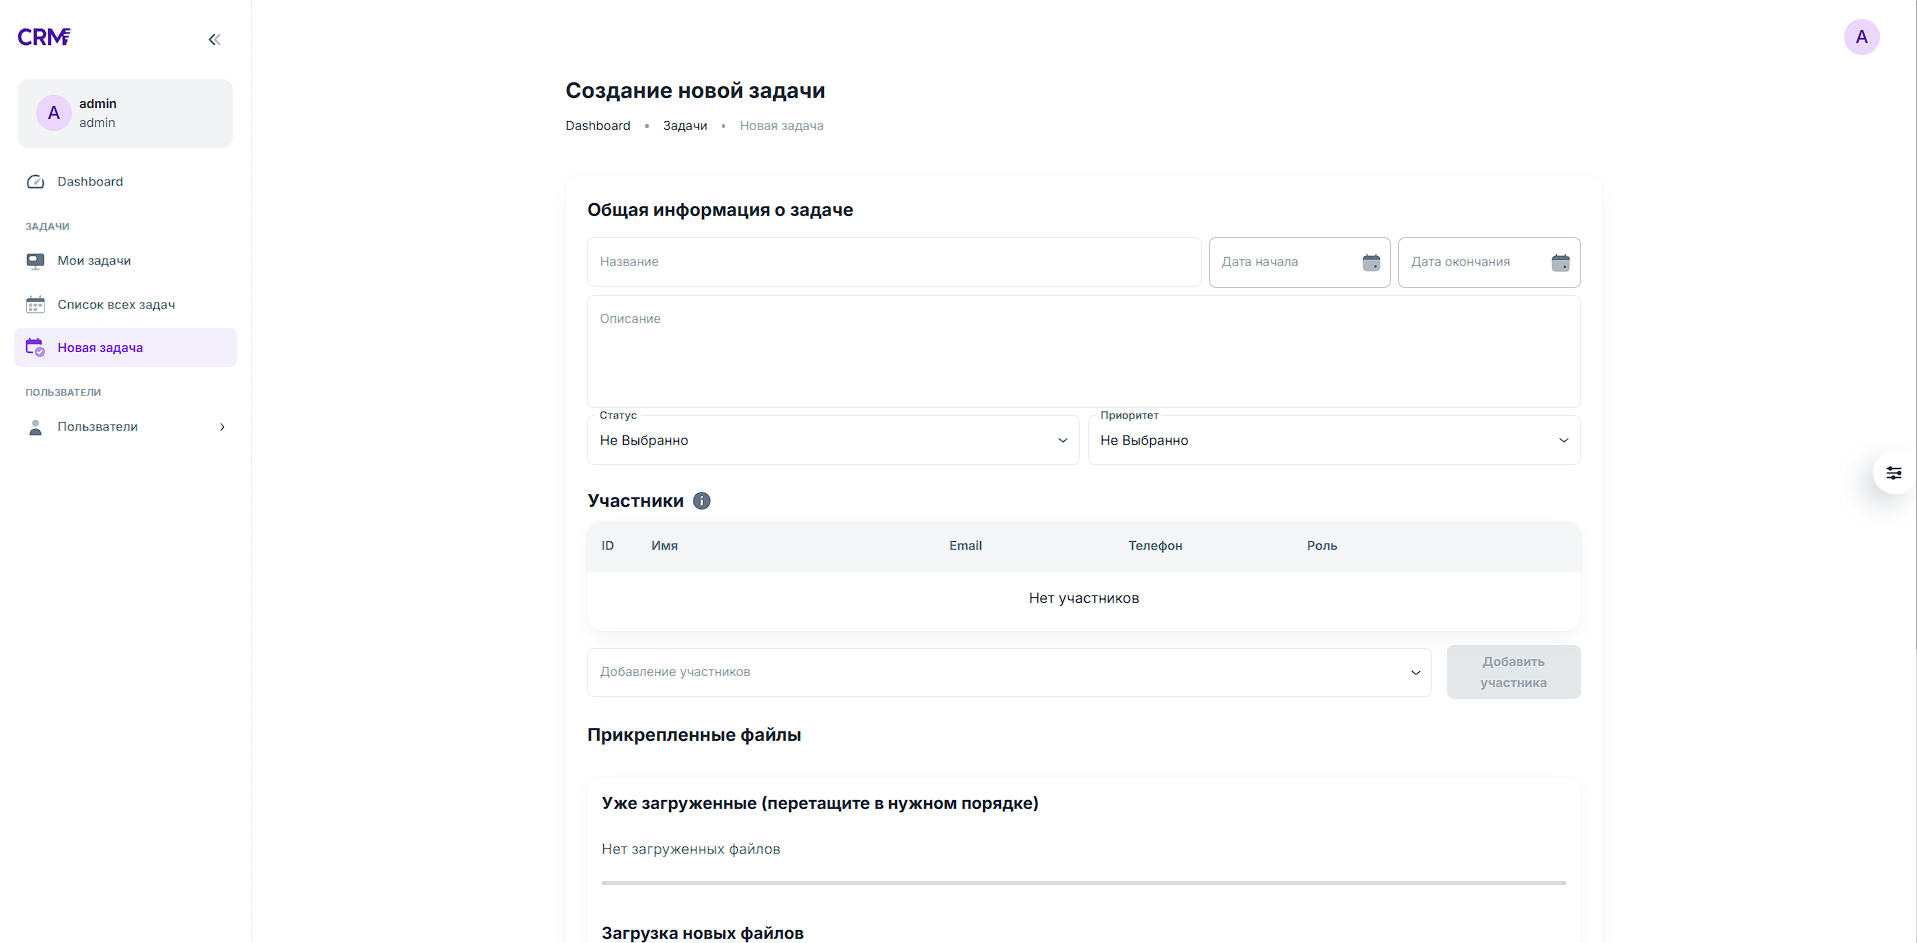
\includegraphics[width=0.75\linewidth]{\commonSecPathPrefix/sec_5/content/task.png}}
    \caption{Страница создания задачи}
    \label{fig:task}
\end{figure}

Основные поля задачи содержат всю информацию о задаче: название, сроки исполнения, приоритет и статус. Блок добавления задачи является
таблицой пользователей, в которую можно добавлять и удалять участников задачи. Блок добавления файлов состоит из двух элементов: выбранные
файлы и зона добавления файла с возможностью перетянуть в неё файл.